% vim: set tw=0:
\documentclass{beamer}
\usepackage{graphicx}
\usepackage{hyperref}
\hypersetup{pdfborder={0 0 0 0}}

% Reasonable themes:
% Antibes Bergen Berkeley Berlin Frankfurt Goettingen Ilmenau Luebeck Malmoe
% Montpellier PaloAlto Rochester Singapore Szeged Warsaw bars boxes
% compatibility default lined plain shadow sidebar split tree
% And these ones include the author's name on every slide:
% Berkeley

% Declare themes.
\mode<presentation>
\usetheme{UWHEP}

% Personal macros.
\newcommand{\email}[1]{{\texttt #1}}
\newcommand{\newframe}[1]{\section{#1}
    \frametitle{\sc{#1}}}
\newcommand{\subframe}[1]{\subsection{#1}
    \frametitle{\sc{#1}}}
\newcommand{\supers}[1]{\ensuremath{^\textrm{#1}}}
\newcommand{\subs}[1]{\ensuremath{_\textrm{#1}}}
\newcommand{\ca}{\ensuremath{\sim}}
\renewcommand{\email}[1]{\href{mailto:#1}{\nolinkurl{#1}}}

% Author information.
\title{T2 Status}
\author[Maier, Mohapatra]{
    Will Maier \and Ajit Mohapatra\\ 
    {\tt wcmaier@hep.wisc.edu}\\
    {\tt ajit@hep.wisc.edu}}
\institute[Wisconsin]{University of Wisconsin - High Energy Physics}
\date{2009.10.27}
\logo{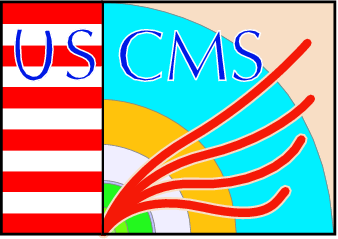
\includegraphics[height=0.6cm]{../../../Graphics/USCMS_logo.png}\hspace{.1cm}
\includegraphics[height=0.75cm]{../../../Graphics/UW_logo.png}}

\begin{document}

\begin{frame}
    \titlepage
\end{frame}

%\section{Overview}
%\begin{frame}
%    \tableofcontents
%\end{frame}

\section{Facilities}
\subsection{Software and Storage}
\begin{frame}
\frametitle{}

\begin{itemize}
	\item 2009.10.27: AFS problems
	\begin{itemize}
		\item UPS overloaded, then a series of kernel panics
	\end{itemize}
	\item 2009.10.25: dCache filled up
	\begin{itemize}
		\item Replacing RECO with AODSIM, planning next storage purchase
	\end{itemize}
	\item Matteo Sani submitted 5k jobs, each running more than a day
	\begin{itemize}
		\item Queues swelled to 7-8k, Sani's jobs didn't make any real progress
		\item Killed them all and suggested resubmitting with shorter run times
	\end{itemize}
	\item Various bug fixes in billingrep, PFM; wrote more tests for {\tt billingrep}
	\item Observed dcap error 'OK'/{\tt dc\_errno=0} on Ken's jobs
	\begin{itemize}
		\item We've also seen this in a very small number of JobRobot failures in the last year
		\item No idea what causes it (or why {\tt dc\_errno=0} means something bad happened)
	\end{itemize}
	\item Lots of disk RMAs
\end{itemize}

\end{frame}

\subsection{Production and Monitoring}
\begin{frame}
\frametitle{}
\begin{itemize}
	\item JobRobot: OK
	\item SAM: Hiccups due to full dCache (2009.10.25-26) and AFS problems (2009.10.27)
	\item RSV: OK
	\item PhEDEx:
	\begin{itemize}
		\item Bug in the data consistency check tool was causing the BlockDownloadVerify component to crash
		\item Communicated with the PhEDEx developers about it and tested the fix which went into 3\_2\_9 release
		\item Updated both our PhEDEx servers to 3\_2\_9 and things running OK
		\item Usual MC sample xfers for local users.
	\end{itemize}
	\item MC Production:
	\begin{itemize}
		\item Summer09 FDMC/FAMC production continues; next round will be LHE/MadGraph production
		\item Dorian (Caltech) will help run production in OSG
		\item Please add Dorian's DN~\footnote{{\tt {\tiny /DC=ch/DC=cern/OU=Organic Units/OU=Users/CN=dkcira/CN=655958/CN=Dorian Kcira}}} so that he can write/read to/from your SE using the {\tt /cms/Role=production} role
	\end{itemize}
\end{itemize}
\end{frame}

\end{document}
